% ============================================================
%  Hybrid GP: GP-Assisted Dyadic Compression
%  Compile: pdflatex hybrid_gp_slides.tex  (run twice)
%  Requires: beamer-theme-metropolis
% ============================================================
\documentclass[aspectratio=169, 10pt]{beamer}

\usetheme{metropolis}

% ── packages ────────────────────────────────────────────────
\usepackage{booktabs}
\usepackage{colortbl}
\usepackage{amsmath, amssymb, bm}
\usepackage{graphicx}
\usepackage{xcolor}
\usepackage{tikz}
\usepackage[protrusion=true, expansion=false]{microtype}
\usepackage[T1]{fontenc}
\usetikzlibrary{arrows.meta, positioning, shapes.geometric, fit,
                backgrounds, calc, decorations.pathreplacing}

\graphicspath{{./}}

% ── colour palette ──────────────────────────────────────────
\definecolor{cnavy}{HTML}{0D2137}
\definecolor{cteal}{HTML}{1A6B8A}
\definecolor{cmint}{HTML}{02C39A}
\definecolor{cice}{HTML}{E4F2F8}
\definecolor{cmid}{HTML}{7BB8CC}
\definecolor{cdgray}{HTML}{2E4057}
\definecolor{camber}{HTML}{F0A500}
\definecolor{cmuted}{HTML}{5A7385}

% ── metropolis overrides ────────────────────────────────────
\setbeamercolor{normal text}{fg=cnavy, bg=white}
\setbeamercolor{frametitle}{bg=cnavy, fg=white}
\setbeamercolor{title separator}{fg=cmint}
\setbeamercolor{progress bar}{fg=cmint, bg=cice}
\setbeamercolor{alerted text}{fg=cmint}
\setbeamercolor{block title}{bg=cice, fg=cnavy}
\setbeamercolor{block body}{bg=cice!40, fg=cnavy}
\setbeamercolor{itemize item}{fg=cteal}
\setbeamercolor{itemize subitem}{fg=cmuted}
\setbeamerfont{frametitle}{size=\large, series=\bfseries}
\setbeamerfont{block title}{series=\bfseries, size=\footnotesize}
\setbeamerfont{block body}{size=\footnotesize}

% tighten vertical spacing globally
\setlength{\parskip}{2pt}

% ── title info ───────────────────────────────────────────────
\title{Hybrid GP: GP-Assisted Dyadic Compression}
\subtitle{for Scientific Data Compression}
\author{Jessie Chen}
\institute{Argonne National Laboratory}
\date{October 2026}

% ── helper: step circle ──────────────────────────────────────
\newcommand{\stepcircle}[1]{%
  \tikz[baseline=-0.6ex]\node[circle, fill=cmint, text=cnavy,
    font=\bfseries\small, inner sep=2.5pt]{#1};}

% ── helper: stat box ─────────────────────────────────────────
\newcommand{\statbox}[3]{%
  \begin{beamercolorbox}[sep=5pt, rounded=true, shadow=false,
      wd=\linewidth]{block body}
    {\scriptsize\color{cmid}\textbf{#1}}\\[1pt]
    {\normalsize\bfseries\color{cnavy} #2}\\[1pt]
    {\tiny\color{cdgray} #3}
  \end{beamercolorbox}}

% ─────────────────────────────────────────────────────────────
\begin{document}

% ── SLIDE 1: Title ───────────────────────────────────────────
{
\setbeamercolor{background canvas}{bg=cnavy}
\setbeamercolor{normal text}{fg=white}
\begin{frame}[plain]
  \vspace{2em}
  {\color{cmint}\rule{3pt}{0.62\textheight}}\hspace{1em}%
  \begin{minipage}{0.88\textwidth}
    \raggedright
    {\fontsize{24}{30}\selectfont\bfseries\color{white}
      Hybrid GP: GP-Assisted\\[4pt]Dyadic Compression}\\[8pt]
    {\large\color{cice} for Scientific Data Compression}\\[24pt]
    {\small\color{cmid}
      ISABEL Hurricane Wf48 \quad
      GP on first 2 dyadic levels \quad
      Switch to cubic spline thereafter}
  \end{minipage}
\end{frame}
}

% ── SLIDE 2: SZ3 Baseline ────────────────────────────────────
\begin{frame}[shrink=5]{SZ3 Interpolation: Dyadic Refinement}
\vspace{0.15em}
\begin{columns}[T, totalwidth=\textwidth]
  \begin{column}{0.52\textwidth}
    {\footnotesize SZ3's \texttt{ALGO\_INTERP} uses a \textbf{dyadic (halving)
    schedule} along each axis.}

    \smallskip
    {\footnotesize\bfseries\color{cteal} Level 0 — coarse grid (stride 32):}\\[1pt]
    {\footnotesize Every 32nd point stored as raw float32.}

    \smallskip
    {\footnotesize\bfseries\color{cteal} Levels 1, 2, \ldots — midpoint fill:}\\[1pt]
    {\footnotesize Each level halves the stride. Midpoints predicted via:
    $\hat{v}_m = (-v_a + 9v_b + 9v_c - v_d)/16$}\\[2pt]
    {\footnotesize Residual $v - \hat{v}$ is quantised and Huffman-coded.}

    \smallskip
    {\scriptsize\color{cmuted}
      Level 5 alone contains \textbf{86\%} of all 25\,M points.\\
      X, Y, Z sweeps at each level; cumulative known set grows.}
  \end{column}

  \begin{column}{0.04\textwidth}
    \color{cteal}\rule{1pt}{0.78\textheight}
  \end{column}

  \begin{column}{0.44\textwidth}
    % Dyadic diagram — compact scale to avoid hbox overflow
    \resizebox{\linewidth}{!}{%
    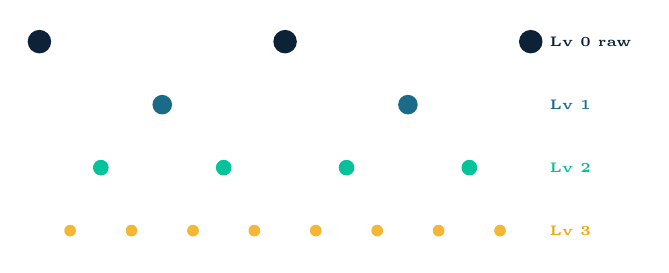
\begin{tikzpicture}[x=0.78cm,y=0.80cm]
      \foreach \x in {0,4,8} {
        \node[circle,fill=cnavy,inner sep=3pt] at (\x,3) {};
      }
      \foreach \x in {2,6} {
        \node[circle,fill=cteal,inner sep=2.5pt] at (\x,2) {};
      }
      \foreach \x in {1,3,5,7} {
        \node[circle,fill=cmint,inner sep=2pt] at (\x,1) {};
      }
      \foreach \x in {0.5,1.5,2.5,3.5,4.5,5.5,6.5,7.5} {
        \node[circle,fill=camber!80,inner sep=1.5pt] at (\x,0) {};
      }
      \node[right,font=\tiny\bfseries,color=cnavy]  at (8.15,3) {Lv 0\ raw};
      \node[right,font=\tiny\bfseries,color=cteal]  at (8.15,2) {Lv 1};
      \node[right,font=\tiny\bfseries,color=cmint]  at (8.15,1) {Lv 2};
      \node[right,font=\tiny\bfseries,color=camber] at (8.15,0) {Lv 3};
    \end{tikzpicture}}
  \end{column}
\end{columns}
\end{frame}

% ── SLIDE 3: Storage Bottlenecks ─────────────────────────────
\begin{frame}{Where SZ3 Spends Its Bits}
\vspace{0.2em}
\begin{columns}[T, totalwidth=\textwidth]

  \begin{column}{0.47\textwidth}
    \begin{block}{\stepcircle{!}\hspace{4pt} Bottleneck 1 — Raw coarse grid}
      \footnotesize
      Level 0 stores \textbf{every} coarse-grid point losslessly.
      At stride 32 on $500{\times}500{\times}100$ this is
      ${\approx}2\text{k}$ points $\times$ 32 bits — a fixed cost
      regardless of data compressibility.
    \end{block}
    \vspace{4pt}
    {\scriptsize\color{cmuted}
      Anchors $\sim$5\% of bits at low EB; dominant at high EB.}
  \end{column}

  \begin{column}{0.06\textwidth}
    \color{cteal}\rule{1pt}{0.72\textheight}
  \end{column}

  \begin{column}{0.47\textwidth}
    \begin{block}{\stepcircle{!}\hspace{4pt} Bottleneck 2 — Poor early predictions}
      \footnotesize
      At levels 1--2 the grid is still sparse. The cubic spline sees
      neighbours 32 points apart $\Rightarrow$ large residuals
      $\Rightarrow$ high-entropy q-bins.
    \end{block}
    \vspace{4pt}
    {\scriptsize\color{cmuted}
      Early levels: $H > 4$ bits/pt; level 5 settles near 2.
      Fixing first few levels shifts the whole RD curve.}
  \end{column}

\end{columns}
\vfill
{\scriptsize\color{cmuted}\itshape
  Both bottlenecks hit the coarse regime — where GP is cheapest to apply.}
\end{frame}

% ── SLIDE 4: Hybrid GP Overview ──────────────────────────────
\begin{frame}{Hybrid GP: the Idea}
\vspace{0.3em}
\begin{columns}[T, totalwidth=\textwidth]

  \begin{column}{0.60\textwidth}
    \resizebox{\linewidth}{!}{%
    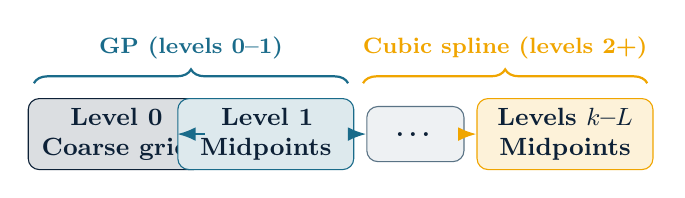
\begin{tikzpicture}[x=1.9cm, y=1.0cm]
      \node[rectangle,rounded corners=4pt,draw=cnavy,fill=cnavy!15,
            text=cnavy,font=\small\bfseries,
            minimum height=0.70cm, text width=2.0cm, align=center]
        (lv0) at (0,0) {Level 0\\Coarse grid};
      \node[rectangle,rounded corners=4pt,draw=cteal,fill=cteal!15,
            text=cnavy,font=\small\bfseries,
            minimum height=0.70cm, text width=2.0cm, align=center]
        (lv1) at (1,0) {Level 1\\Midpoints};
      \node[rectangle,rounded corners=4pt,draw=cmuted,fill=cmuted!10,
            text=cnavy,font=\small\bfseries,
            minimum height=0.70cm, text width=1.0cm, align=center]
        (dots) at (2,0) {\ldots};
      \node[rectangle,rounded corners=4pt,draw=camber,fill=camber!15,
            text=cnavy,font=\small\bfseries,
            minimum height=0.70cm, text width=2.0cm, align=center]
        (end) at (3,0) {Levels $k$--$L$\\Midpoints};
      \draw[-Latex,thick,color=cteal]  (lv0) -- (lv1);
      \draw[-Latex,thick,color=cteal]  (lv1) -- (dots);
      \draw[-Latex,thick,color=camber] (dots) -- (end);
      \draw[thick,color=cteal,decorate,
            decoration={brace,amplitude=5pt,raise=7pt}]
        (-0.55,0.40) -- (1.55,0.40)
        node[midway,above=12pt,font=\footnotesize\bfseries,color=cteal]
          {GP (levels 0--1)};
      \draw[thick,color=camber,decorate,
            decoration={brace,amplitude=5pt,raise=7pt}]
        (1.65,0.40) -- (3.55,0.40)
        node[midway,above=12pt,font=\footnotesize\bfseries,color=camber]
          {Cubic spline (levels 2+)};
    \end{tikzpicture}}

    \vspace{0.5em}
    {\scriptsize\color{cmuted}
      \textbf{GP\_LEVELS}\,=\,2: levels 0 and 1 use GP.
      All remaining levels use SZ3 cubic spline verbatim.}
  \end{column}

  \begin{column}{0.04\textwidth}
    \color{cteal}\rule{1pt}{0.62\textheight}
  \end{column}

  \begin{column}{0.36\textwidth}
    {\footnotesize\bfseries\color{cteal} GP phase}\\[3pt]
    {\footnotesize Fit HPs on true values; RPCholesky selects sparse
    anchors; full GP predicts the rest; residuals quantised to
    $\pm\varepsilon_b$.}

    \medskip
    {\footnotesize\bfseries\color{camber} Cubic phase}\\[3pt]
    {\footnotesize SZ3 4-point cubic, O(N). Identical to
    \texttt{ALGO\_INTERP} from level 2 onward.}
  \end{column}

\end{columns}
\end{frame}

% ── SLIDE 5: Level 0 ─────────────────────────────────────────
\begin{frame}{Level 0 — Coarse Grid via GP}
\vspace{0.15em}
\begin{columns}[T, totalwidth=\textwidth]

  \begin{column}{0.50\textwidth}
    \stepcircle{1}\enspace{\footnotesize\bfseries\color{cteal} Fit hyperparameters}\\[1pt]
    \hspace{1.5em}{\footnotesize Matérn-5/2 MLE on 800-pt subsample
      $\to$ \texttt{ls\_xy}, \texttt{ls\_z}, $\sigma^2$}

    \smallskip
    \stepcircle{2}\enspace{\footnotesize\bfseries\color{cteal} Select anchors (RPCholesky)}\\[1pt]
    \hspace{1.5em}{\footnotesize $\alpha{=}5\%$ of coarse-grid points
      selected; stored as raw float32.}

    \smallskip
    \stepcircle{3}\enspace{\footnotesize\bfseries\color{cteal} GP predict remaining 95\%}\\[1pt]
    \hspace{1.5em}{\footnotesize Full Cholesky on anchor set
      (${\sim}100$ pts, feasible). Predict all non-anchor coarse pts.}

    \smallskip
    \stepcircle{4}\enspace{\footnotesize\bfseries\color{cteal} Quantise}\\[1pt]
    \hspace{1.5em}{\footnotesize
      $q = \mathrm{round}\!\left(\frac{v - \hat{v}}{2\varepsilon_b}\right)$
      $\Rightarrow$ recon within $\pm\varepsilon_b$.}

    \vspace{4pt}
    {\scriptsize\color{cmuted}
      Same $\pm\varepsilon_b$ guarantee as SZ3.}
  \end{column}

  \begin{column}{0.04\textwidth}
    \color{cteal}\rule{1pt}{0.78\textheight}
  \end{column}

  \begin{column}{0.46\textwidth}
    % Anchor scatter diagram (6x4 grid)
    \resizebox{0.85\linewidth}{!}{%
    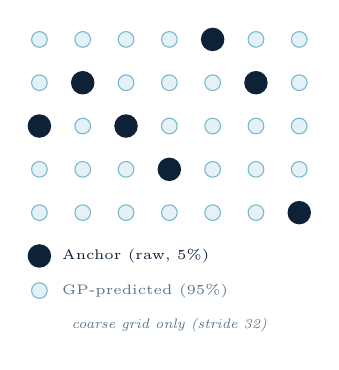
\begin{tikzpicture}[x=0.55cm,y=0.55cm]
      \foreach \x in {0,1,2,3,4,5,6} {
        \foreach \y in {0,1,2,3,4} {
          \node[circle,fill=cice,draw=cmid,inner sep=2pt] at (\x,\y) {};
        }
      }
      \node[circle,fill=cnavy,inner sep=3pt] at (1,3) {};
      \node[circle,fill=cnavy,inner sep=3pt] at (3,1) {};
      \node[circle,fill=cnavy,inner sep=3pt] at (5,3) {};
      \node[circle,fill=cnavy,inner sep=3pt] at (6,0) {};
      \node[circle,fill=cnavy,inner sep=3pt] at (0,2) {};
      \node[circle,fill=cnavy,inner sep=3pt] at (4,4) {};
      \node[circle,fill=cnavy,inner sep=3pt] at (2,2) {};
      % Legend
      \node[circle,fill=cnavy,inner sep=3pt] at (0,-1.0) {};
      \node[right,font=\tiny,color=cnavy] at (0.3,-1.0) {Anchor (raw, 5\%)};
      \node[circle,fill=cice,draw=cmid,inner sep=2pt] at (0,-1.8) {};
      \node[right,font=\tiny,color=cmuted] at (0.3,-1.8) {GP-predicted (95\%)};
      \node[font=\tiny\itshape,color=cmuted,align=center] at (3,-2.6)
        {coarse grid only (stride 32)};
    \end{tikzpicture}}
  \end{column}

\end{columns}
\end{frame}

% ── SLIDE 6: Level 1 ─────────────────────────────────────────
\begin{frame}{Level 1 — First Midpoints via GP}
\vspace{0.15em}
\begin{columns}[T, totalwidth=\textwidth]

  \begin{column}{0.50\textwidth}
    \stepcircle{1}\enspace{\footnotesize\bfseries\color{cteal} Per-level HP fitting}\\[1pt]
    \hspace{1.5em}{\footnotesize Fit HPs on true values at level-1 positions.}

    \smallskip
    \stepcircle{2}\enspace{\footnotesize\bfseries\color{cteal} Full GP prediction}\\[1pt]
    \hspace{1.5em}{\footnotesize Condition on all resolved level-0 points.
      Predict all new midpoints in one solve.}

    \smallskip
    \stepcircle{3}\enspace{\footnotesize\bfseries\color{cteal} Quantise \& extend}\\[1pt]
    \hspace{1.5em}{\footnotesize Residuals quantised to $\pm\varepsilon_b$.
      Reconstructed values join the conditioning set.}

    \vspace{4pt}
    {\scriptsize\color{cmuted}
      Sweep order (X $\to$ Y $\to$ Z) mirrors SZ3 exactly.}
  \end{column}

  \begin{column}{0.04\textwidth}
    \color{cteal}\rule{1pt}{0.78\textheight}
  \end{column}

  \begin{column}{0.46\textwidth}
    % 1-D dyadic grid slice
    \resizebox{0.90\linewidth}{!}{%
    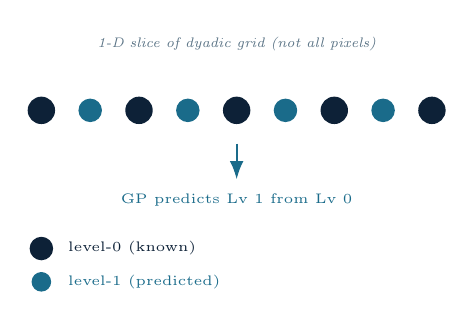
\begin{tikzpicture}[x=0.62cm,y=0.65cm]
      \node[font=\tiny\itshape,color=cmuted,align=center] at (4,4.8)
        {1-D slice of dyadic grid (not all pixels)};
      \foreach \x in {0,2,4,6,8} {
        \node[circle,fill=cnavy,inner sep=3.5pt] at (\x,3.5) {};
      }
      \foreach \x in {1,3,5,7} {
        \node[circle,fill=cteal,inner sep=3pt] at (\x,3.5) {};
      }
      \draw[-Latex,thick,color=cteal] (4,2.85) -- (4,2.15);
      \node[font=\tiny,color=cteal,align=center] at (4,1.75)
        {GP predicts Lv 1 from Lv 0};
      \node[circle,fill=cnavy,inner sep=3pt] at (0,0.8) {};
      \node[right,font=\tiny,color=cnavy] at (0.35,0.8) {level-0 (known)};
      \node[circle,fill=cteal,inner sep=2.5pt] at (0,0.15) {};
      \node[right,font=\tiny,color=cteal] at (0.35,0.15) {level-1 (predicted)};
    \end{tikzpicture}}
  \end{column}

\end{columns}
\end{frame}

% ── SLIDE 7: Handoff to Cubic Spline ─────────────────────────
\begin{frame}[shrink=5]{Switching to Cubic Spline at Level 2}
\vspace{0.15em}
\begin{columns}[T, totalwidth=\textwidth]

  \begin{column}{0.55\textwidth}
    {\footnotesize From level 2 onward: \textbf{identical} to SZ3 \texttt{ALGO\_INTERP}.}

    \smallskip
    \stepcircle{1}\enspace{\footnotesize\bfseries\color{camber} 4-point cubic}\\[1pt]
    \hspace{1.5em}{\footnotesize $(-v_a + 9v_b + 9v_c - v_d)/16$;
    linear at boundaries.}

    \smallskip
    \stepcircle{2}\enspace{\footnotesize\bfseries\color{camber} Quantise \& update}\\[1pt]
    \hspace{1.5em}{\footnotesize Quantise residual; write to \texttt{vol\_recon};
    extend cumulative set.}

    \smallskip
    \stepcircle{3}\enspace{\footnotesize\bfseries\color{camber} X $\to$ Y $\to$ Z sweeps}\\[1pt]
    \hspace{1.5em}{\footnotesize Repeat per dimension until all 25\,M points resolved.}

    \medskip
    {\footnotesize GP-resolved base $\Rightarrow$ smaller cubic residuals
    $\Rightarrow$ lower entropy $\Rightarrow$ fewer bits.}
  \end{column}

  \begin{column}{0.04\textwidth}
    \color{cteal}\rule{1pt}{0.72\textheight}
  \end{column}

  \begin{column}{0.41\textwidth}
    \resizebox{0.82\linewidth}{!}{%
    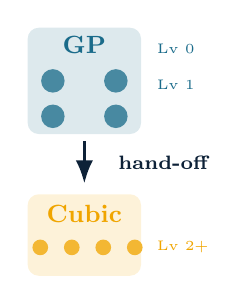
\begin{tikzpicture}[x=0.8cm,y=0.9cm]
      \fill[cteal!15,rounded corners=4pt] (-0.4,1.8) rectangle (1.4,3.3);
      \node[font=\small\bfseries,color=cteal] at (0.5,3.05) {GP};
      \node[circle,fill=cteal!80,inner sep=3pt] at (0,2.55) {};
      \node[circle,fill=cteal!80,inner sep=3pt] at (1,2.55) {};
      \node[circle,fill=cteal!80,inner sep=3pt] at (0,2.05) {};
      \node[circle,fill=cteal!80,inner sep=3pt] at (1,2.05) {};
      \draw[-Latex,very thick,color=cnavy] (0.5,1.70) -- (0.5,1.10);
      \node[font=\scriptsize\bfseries,color=cnavy] at (1.75,1.40) {hand-off};
      \fill[camber!15,rounded corners=4pt] (-0.4,-0.2) rectangle (1.4,0.95);
      \node[font=\small\bfseries,color=camber] at (0.5,0.68) {Cubic};
      \node[circle,fill=camber!80,inner sep=2pt] at (-0.2,0.20) {};
      \node[circle,fill=camber!80,inner sep=2pt] at (0.3,0.20) {};
      \node[circle,fill=camber!80,inner sep=2pt] at (0.8,0.20) {};
      \node[circle,fill=camber!80,inner sep=2pt] at (1.3,0.20) {};
      \node[right,font=\tiny,color=cteal]  at (1.5,3.0) {Lv 0};
      \node[right,font=\tiny,color=cteal]  at (1.5,2.5) {Lv 1};
      \node[right,font=\tiny,color=camber] at (1.5,0.2) {Lv 2+};
    \end{tikzpicture}}

    \vspace{4pt}
    {\scriptsize\color{cmuted}
      Cubic phase is O(N).\\
      Level 5 = 86\% of all points.}
  \end{column}

\end{columns}
\end{frame}

% ── SLIDE 8: Algorithm Summary ───────────────────────────────
\begin{frame}[shrink=8]{Algorithm — Hybrid GP}
\vspace{0.1em}
\begin{columns}[T, totalwidth=\textwidth]

  \begin{column}{0.47\textwidth}
    {\footnotesize\bfseries\color{cteal} Init}\\[1pt]
    \hspace{0.6em}{\footnotesize\textbf{1.} Load $v$, z-score normalise.
    Build schedules $\mathcal{S}_x, \mathcal{S}_y, \mathcal{S}_z$.}

    \smallskip
    {\footnotesize\bfseries\color{cteal} Level 0}\\[1pt]
    \hspace{0.6em}{\footnotesize\textbf{2.} Collect $S$ coarse pts; fit HPs via MLE.}\\[1pt]
    \hspace{0.6em}{\footnotesize\textbf{3.} RPCholesky: $\lfloor\alpha S\rfloor$ anchors $\to$ float32.}\\[1pt]
    \hspace{0.6em}{\footnotesize\textbf{4.} GP predicts remaining $S{-}\lfloor\alpha S\rfloor$ pts.}\\[1pt]
    \hspace{0.6em}{\footnotesize\textbf{5.} Quantise: $q{=}\mathrm{round}((v{-}\hat{v})/(2\varepsilon_b))$.}

    \smallskip
    {\footnotesize\bfseries\color{cteal} Level 1}\\[1pt]
    \hspace{0.6em}{\footnotesize\textbf{6.} Collect midpoints; fit per-level HPs.}\\[1pt]
    \hspace{0.6em}{\footnotesize\textbf{7.} GP conditioned on all resolved pts.}\\[1pt]
    \hspace{0.6em}{\footnotesize\textbf{8.} Quantise; add to conditioning set.}
  \end{column}

  \begin{column}{0.06\textwidth}
    \color{cteal}\rule{1pt}{0.80\textheight}
  \end{column}

  \begin{column}{0.47\textwidth}
    {\footnotesize\bfseries\color{camber} Levels 2+}\\[1pt]
    \hspace{0.6em}{\footnotesize\textbf{9.}  X/Y/Z sweep: 4-point cubic formula.}\\[1pt]
    \hspace{0.6em}{\footnotesize\textbf{10.} Quantise; update \texttt{vol\_recon}.}\\[1pt]
    \hspace{0.6em}{\footnotesize\textbf{11.} Extend cumulative set. Repeat.}

    \smallskip
    {\footnotesize\bfseries\color{cteal} Output}\\[1pt]
    \hspace{0.6em}{\footnotesize\textbf{12.} Entropy-code q-bins (Huffman).}\\[1pt]
    \hspace{0.6em}{\footnotesize\textbf{13.} Write anchors + raw values + stream.}

    \medskip
    \begin{block}{Parameters}
      \footnotesize
      \texttt{GP\_LEVELS} = 2\quad\texttt{ANCHOR\_FRAC} = 5\%\\
      \texttt{INIT\_STRIDE} = 32\quad\texttt{NOISE} = $10^{-4}$\\
      Kernel: anisotropic Matérn-5/2
    \end{block}
  \end{column}

\end{columns}
\end{frame}

% ── SLIDE 9: Error Bound ─────────────────────────────────────
\begin{frame}{Error Bound: Same Guarantee as SZ3}
\vspace{0.2em}
\begin{columns}[T, totalwidth=\textwidth]

  \begin{column}{0.47\textwidth}
    \begin{block}{Quantisation ensures $\pm\varepsilon_b$}
      \footnotesize
      For every predicted point $i$:
      \[
        q_i = \left\lfloor \frac{v_i - \hat{v}_i}{2\varepsilon_b}
              \right\rceil, \quad
        v_i^{\mathrm{recon}} = \hat{v}_i + q_i \cdot 2\varepsilon_b
      \]
      $|v_i - v_i^{\mathrm{recon}}| \le \varepsilon_b$ regardless of
      GP quality.
    \end{block}

    \smallskip
    {\footnotesize Better GP predictions $\Rightarrow$ smaller $|q_i|$
    $\Rightarrow$ lower entropy $\Rightarrow$ fewer bits.}
  \end{column}

  \begin{column}{0.06\textwidth}
    \color{cteal}\rule{1pt}{0.72\textheight}
  \end{column}

  \begin{column}{0.47\textwidth}
    {\footnotesize\bfseries\color{cteal} Error propagation}\\[3pt]
    {\footnotesize Level-1+ conditions on level-0 reconstructions
    (within $\pm\varepsilon_b$). Quantisation clamps total error
    to $\pm\varepsilon_b$ regardless.}

    \medskip
    {\footnotesize\bfseries\color{cteal} Why GP helps}\\[3pt]
    {\footnotesize At level 1, cubic spline neighbours are 32 grid
    points apart. GP exploits global correlation and best-placed
    anchors $\Rightarrow$ smaller $|q_i|$.}
  \end{column}

\end{columns}
\end{frame}

% ── SLIDE 10: Per-Level Bit Breakdown ────────────────────────
\begin{frame}{Per-Level Bit Breakdown (EB $= 0.01$)}
\vspace{0.2em}

{\footnotesize GP levels 0--1 contribute $<1\%$ of total bits, yet their
quality propagates to all subsequent cubic levels.}

\smallskip
{\footnotesize
\begin{tabular}{lrrrrrr}
  \toprule
  Level & Method & N pts & $H$ (bits) & \% of total & \% $|q|{\le}1$ \\
  \midrule
  —    & Anchors   & 100   & 32.0 & ${\sim}0.1\%$ & 100\% \\
  0    & GP        & 2\,k  & low  & ${\sim}0.0\%$ & high  \\
  1    & GP        & 15\,k & low  & ${\sim}0.5\%$ & high  \\
  2    & Cubic     & 60\,k & med  & ${\sim}2\%$   & med   \\
  3--4 & Cubic     & 500\,k & med & ${\sim}10\%$  & med   \\
  5    & Cubic     & 21\,M & low  & ${\sim}86\%$  & high  \\
  \bottomrule
\end{tabular}
}

\smallskip
{\scriptsize\color{cmuted}
  Level 5 dominates (86\% of all 25\,M pts). GP foundation $\Rightarrow$
  smaller cubic residuals at fine levels $\Rightarrow$ lower overall entropy.
  Numbers approximate from pilot runs.}
\end{frame}

% ── SLIDE 11: Experiment Setup ───────────────────────────────
\begin{frame}{Experiment Setup}
\vspace{0.2em}
\begin{columns}[T, totalwidth=\textwidth]

  \begin{column}{0.47\textwidth}
    \begin{block}{Dataset}
      \footnotesize
      Hurricane ISABEL W (Wf48)\\
      Grid: $500 \times 500 \times 100$\ (25\,M float32)\\
      EB: 0.005, 0.01, 0.02, 0.05, 0.1
    \end{block}

    \medskip
    \begin{block}{Hybrid GP config}
      \footnotesize
      \texttt{GP\_LEVELS}\,=\,2\ (levels 0--1 use GP)\\
      \texttt{ANCHOR\_FRAC}\,=\,5\%\ of coarse grid\\
      \texttt{INIT\_STRIDE}\,=\,32\\
      Kernel: Matérn-5/2, anisotropic\\
      HP fit: L-BFGS-B MLE, 800-pt sample
    \end{block}
  \end{column}

  \begin{column}{0.06\textwidth}
    \color{cteal}\rule{1pt}{0.72\textheight}
  \end{column}

  \begin{column}{0.47\textwidth}
    \begin{block}{Baseline}
      \footnotesize
      SZ3 \texttt{ALGO\_INTERP} (same EB values)\\
      Official binary, default settings
    \end{block}

    \medskip
    \begin{block}{Metrics}
      \footnotesize
      Bit rate (bpv) = total bits / 25\,M\\
      PSNR (dB) $= 20\log_{10}(\Delta/\mathrm{RMSE})$\\
      CR $= 32 / \mathrm{bpv}$\quad Wall-clock time (s)
    \end{block}
  \end{column}

\end{columns}
\end{frame}

% ── SLIDE 12: RD Curve ───────────────────────────────────────
\begin{frame}{Rate–Distortion Results — Hurricane ISABEL Wf48}
\vspace{0.1em}
\begin{columns}[T, totalwidth=\textwidth]
  \begin{column}{0.60\textwidth}
    \begin{center}
    \includegraphics[width=\linewidth,height=0.68\textheight,
                     keepaspectratio]{rd_hybrid_gp.png}
    \end{center}
  \end{column}
  \begin{column}{0.40\textwidth}
    \vspace{0.5em}
    {\footnotesize\bfseries\color{cteal} Reading the curve}\\[3pt]
    {\footnotesize Higher PSNR at same bit rate = better compression.
    Hybrid GP curve above SZ3-Interp confirms the GP base improves
    cubic quality at all EB levels.}

    \medskip
    {\footnotesize\bfseries\color{cteal} Gain analysis}\\[3pt]
    {\footnotesize Largest gains at mid-range EB (0.01--0.05).
    At very low EB the fine levels dominate and the GP advantage narrows.}

    \vspace{4pt}
    {\scriptsize\color{cmuted}
      Run \texttt{hurricane\_hybrid\_gp.py} to generate the figure.}
  \end{column}
\end{columns}
\end{frame}

% ── SLIDE 13: Timing ─────────────────────────────────────────
\begin{frame}{Timing Comparison}
\vspace{0.2em}
\begin{columns}[T, totalwidth=\textwidth]

  \begin{column}{0.47\textwidth}
    \begin{block}{Where Hybrid GP spends time}
      \footnotesize
      \textbf{Lv 0}: HP fit (${\sim}1$ s) + RPCholesky + Cholesky on
      ${\sim}100$ anchors.\\[3pt]
      \textbf{Lv 1}: HP fit on ${\sim}15$\,k pts (${\sim}2$ s) +
      Cholesky on ${\sim}2$\,k cond.\ set.\\[3pt]
      \textbf{Lv 2+}: O(N) cubic — same speed as SZ3.
    \end{block}
  \end{column}

  \begin{column}{0.06\textwidth}
    \color{cteal}\rule{1pt}{0.58\textheight}
  \end{column}

  \begin{column}{0.47\textwidth}
    \begin{block}{Estimated overhead vs SZ3}
      \footnotesize
      \begin{tabular}{lr}
        \toprule
        Phase & Time \\
        \midrule
        SZ3-Interp baseline  & ${\sim}5$ s \\
        HP fitting (lv 0--1) & $+$3--5 s \\
        RPCholesky + GP solves & $+$2 s \\
        \midrule
        Hybrid GP total      & ${\sim}10$--12 s \\
        \bottomrule
      \end{tabular}
    \end{block}
    \vspace{3pt}
    {\scriptsize\color{cmuted}
      ${\approx}2\times$ wall-clock vs SZ3; GP portion parallelises.}
  \end{column}

\end{columns}
\end{frame}

% ── SLIDE 14: Summary & Next Steps ───────────────────────────
{
\setbeamercolor{background canvas}{bg=cnavy}
\setbeamercolor{frametitle}{bg=cdgray, fg=white}
\begin{frame}{Summary \& Next Steps}
\begin{columns}[T, totalwidth=\textwidth]

  \begin{column}{0.47\textwidth}
    \begin{itemize}\setlength\itemsep{9pt}
      \item[\textcolor{cmint}{$\checkmark$}]
            \textcolor{white}{GP on first 2 dyadic levels:
            only 5\% raw anchors (vs 100\%) and tighter
            early-level residuals}
      \item[\textcolor{cmint}{$\checkmark$}]
            \textcolor{white}{Error bound $\pm\varepsilon_b$
            preserved identically to SZ3}
      \item[\textcolor{cmint}{$\checkmark$}]
            \textcolor{white}{Seamless handoff: levels 2+
            identical to SZ3 \texttt{ALGO\_INTERP}}
    \end{itemize}
  \end{column}

  \begin{column}{0.06\textwidth}
    \color{cteal}\rule{1pt}{0.72\textheight}
  \end{column}

  \begin{column}{0.47\textwidth}
    {\bfseries\color{cmid} Next Steps}\smallskip
    \begin{itemize}\setlength\itemsep{9pt}
      \item[\textcolor{cmint}{$\to$}]
            \textcolor{white}{Adaptive GP\_LEVELS: switch to cubic
            when mean $|q| < \theta$}
      \item[\textcolor{cmint}{$\to$}]
            \textcolor{white}{RPCholesky at level 1+ as well}
      \item[\textcolor{cmint}{$\to$}]
            \textcolor{white}{RD benchmark: Miranda, Nyx, RTM
            with full Huffman encoding}
      \item[\textcolor{cmint}{$\to$}]
            \textcolor{white}{Scale to cluster; combine with
            Patch GP}
    \end{itemize}
  \end{column}

\end{columns}
\end{frame}
}

\end{document}
